\chapter{Analysis of existing methods}

  \section{Problem setup}

    \paragraph{}
    In this part we are going to set the mathematical framework for this study.
    We will start from a partial differential equation arising from the physical model, in the form of
    \begin{equation}\label{eq:pde}
      \frac{\partial \xi}{\partial t} + \operatorname{F}\left(\xi\right) = 0
    \end{equation}
    where the function $\operatorname{F}$ uses some space derivatives of the state variable $\xi$.
    This equation then describe the temporal evolution of the state variables $\xi$.

    \paragraph{}
    A particular class of such partial differential equations are conservative equations.
    They correspond to the case where the function $\operatorname{F}$ can be written as a divergence term.
    Finally, with a source term $\operatorname{S}$, those equations look like:
    \begin{equation}\label{eq:pde_conservative}
      \frac{\partial \xi}{\partial t} + \nabla \cdot \vec{\operatorname{f}}\left(\xi\right) = \operatorname{S}\ .
    \end{equation}
    One might notice that equation (\ref{eq:pde_conservative}) is indeed a particularisation of equation (\ref{eq:pde}), with $\operatorname{F}\left(\xi\right) = \nabla\cdot \vec{\operatorname{f}}\left(\xi\right) - \operatorname{S}$.
    Those conservative equations are the one we will focus on is this study, as they describe the physical systems we are interested in.

    \paragraph{}
    In this work, we will talk about computational fluid dynamics.
    We are in fact mostly interested in the Navier--Stokes equation, and its variants: the reactive Navier--Stokes equation, the Reynold-averaged Navier--Stokes equation, etc.
    A simple form of this equation can be:
    \begin{equation}\label{eq:ns}
      \left\{\begin{aligned}
        &\partial_t\left(\rho         \right) &&+ \nabla\cdot\left( \rho \vec{u} \right) &&= 0 \\
        &\partial_t\left(\rho \vec{u} \right) &&+ \nabla\cdot\left( \rho \vec{u} \otimes \vec{u} + p \id \right) &&= \nabla\cdot \mat{\tau}\\
        &\partial_t\left( \rho E      \right) &&+ \nabla\cdot\left( \left(\rho E + p\right) \vec{u} \right) &&=
          \nabla\cdot\left( \mat{\tau} \cdot \vec{u} \right)
      \end{aligned}\right.
    \end{equation}
    with the \PS{relation de fermeture} $\rho E = \frac{p}{\gamma - 1} + \rho\frac{\vec{u} \cdot \vec{u}}{2}$.
    The deviatoric stress tensor $\tau$ accounts for the viscosity of the fluid, and its computation depends on the model used.
    Without it, one recovers the Euler equations.
    To this simple form can be added source terms from the reactive model, source terms from the turbulence model, divergence terms from a diffusive model, etc.
    Yet it is clear that with a bit of rewriting, we can go back to the starting form (\ref{eq:pde}) and even the conservative form with source terms (\ref{eq:pde_conservative}).
    The quantity $\xi$ is no longer a scalar but a vector with the density $\rho$, each component of the momentum $\rho\vec{u}$ and the energy $\rho E$ as its components.
    Apart from this small change, the idea is the same.

    \paragraph{}
    When solving numerically equations like (\ref{eq:pde}), one must first take a spatial domain on interest.
    Let us call this domain $\mathcal{D}$.
    As we are interested in solving equations numerically, we need to be able to represent different quantities, such as the state variable $\xi$, numerically over the domain $\mathcal{D}$ and store it in the memory of a computer.
    Therefore we need to discretise the continuous spatial domain into a finite number of cells, or elements.
    This is usually done with a mesh of the domain $\mathcal{D}$.
    First we divide the domain $\mathcal{D}$ in a set of cells, called a mesh.
    Those cells are small volumes in 3D, faces in 2D or segments in 1D, disjoints, such as their union recovers the original domain.
    Interest quantities, such as the fluid velocity, density, \dots, are then stored at each nodes, averaged in the center of each cells or sometimes in a more complex fashion depending on the method.
    They are no longer mathematically represented by a function of the continuous physical domain $\xi : \mathcal{D} \rightarrow \mathbb{R}$ but by a finite sized vector $\Xi$ gathering all the information across the discretised domain.
    For some simple discretisation methods, this vector consists of the quantity evaluated at the mesh nodes or averaged at the center of the cells.
    For more complex methods, this vector consists of information used to construct the solution over the domain: polynomial coefficients, spectral decomposition coefficients, etc.
    Anyway, we no longer work in a continuous domain $\mathcal{D}$ but on a discretised one.

    \paragraph{}
    The partial differential equation (\ref{eq:pde}) transforms then into an ordinary differential equation:
    \begin{equation}\label{eq:ode}
      \frac{\partial \Xi}{\partial t} + \operatorname{G}\left(\Xi\right) = 0 \ .
    \end{equation}
    The difference here is that the function $\operatorname{G}$ is a function of a discrete vector whereas $\operatorname{F}$ was a function of a continuous function, and therefore $\operatorname{G}$ does not uses any spatial derivatives.
    Thanks to the spatial discretisation method, the only derivative remaining is with regard to time.
    The rest is then up to the temporal integration method, which is the main topic of this thesis.
    We will work from equation (\ref{eq:ode}) no matter where the function $\operatorname{G}$ comes from, but sometimes understanding the origin of this function can help so we will now introduce the spatial discretisation method used in our solver.


  \section{Brief introduction to the spatial integration schemes}

    \paragraph{}
    A \emph{spatial discretisation method} is the choice of how to represent a quantity over a discretised domain, and how to compute spatial derivative of this quantity from this representation.
    Indeed, before solving equation (\ref{eq:pde}) we need to decide how to transform the continuous model into a discretised one.
    We also have to look at how the spatial derivatives arising from equation (\ref{eq:pde}) translate in the discretised model.

    \subsection{The Finite Volumes method}

      \paragraph{}
      The spatial discretisation method used in the solver CHARME is called the Finite Volumes method \cite{EymardGallouetHerbin2000, Leterrier2003}.
      This method is particularly well fitted for conservatives equations such as equation (\ref{eq:pde_conservative}).
      Such equation has the property that the quantity $\xi$ is conserved: without source terms, the variation of the total quantity on $\xi$ over the domain $\mathcal{D}$ is equal to the flux $f\left(\xi\right)$ coming through the boundary $\partial\mathcal{D}$.
      In the case of the Navier--Stokes equations (\ref{eq:ns}), the density, the momentum and the energy are conserved throughout time, apart from what comes in and out of the domain.
      In a close domain where nothing comes in or out, they are indeed conserved.
      The main interest of the Finite Volumes method is that this property stays true through the spatial discretisation step.

      \paragraph{}
      The Finite Volumes method consists in integrating the partial differential equation over each cell of the mesh.
      Writing $\mathcal{V}_i$ the volume of the $i$th cell:
      \begin{equation}
        \int_{\mathcal{V}_i} \frac{\partial \xi}{\partial t} \mathrm{d}v + \int_{\mathcal{V}_i} \nabla\cdot \vec{\operatorname{f}}\left(\xi\right) \mathrm{d}v = \int_{\mathcal{V}_i} \operatorname{S} \mathrm{d}v\ .
      \end{equation}
      Then the Green--Ostrogradski theorem transforms the flux divergence into a \PS{bilan surfacique}:
      \begin{equation}
        \frac{\mathrm{d}}{\mathrm{d} t} \int_{\mathcal{V}_i} \xi\mathrm{d}v + \oint_{\partial\mathcal{V}_i} \vec{\operatorname{f}}\left(\xi\right) \cdot \vec{\mathrm{d}s} = \int_{\mathcal{V}_i} \operatorname{S} \mathrm{d}v\ .
      \end{equation}
      By writing $\square_i = \frac{1}{\norm{\mathcal{V}_i}} \int_{\mathcal{V}_i} \square \mathrm{d}v$ the average in the $i$th cell, we then have:
      \begin{equation}
        \frac{\mathrm{d}\xi_i}{\mathrm{d} t}  + \frac{1}{\norm{\mathcal{V}_i}} \oint_{\partial\mathcal{V}_i} \vec{\operatorname{f}}\left(\xi\right) \cdot \vec{\mathrm{d}s} = \operatorname{S}_i \ .
      \end{equation}

      \paragraph{}
      As stated before, the spatial discretisation method do transform the partial differential equation into an ordinary differential equation.
      It tells us to store our quantities as the averaged values represented at the center of gravity of each cells as our vector $\Xi$.
      It also tells us to compute the divergence from equation (\ref{eq:pde_conservative}) as a \PS{bilan surfacique de flux}.
      The last thing to do is to decide how to compute this \PS{bilan surfacique de flux}.
      The cells from our meshes are polygons.
      Therefore they have a finite number of (planar) faces.
      The integral over the boundary of the cell can be decomposed by the faces, to get the approximation:
      \begin{equation}
        \oint_{\partial\mathcal{V}_i} \vec{\operatorname{f}}\left(\xi\right) \cdot \vec{\mathrm{d}s} \approx \sum_{j\textrm{ neighbor of } i} \vec{\operatorname{f}}_{ij} \cdot \vec{s_{ij}}
      \end{equation}
      where $\vec{\operatorname{f}}_{ij} \cdot \vec{s_{ij}}$ is an approximation of the flux going through the face between cells $i$ and $j$.
      This approximation is a key element of the Finite Volumes method, therefore we will discuss it later.
      We can now compute the function $\operatorname{G}$ from equation (\ref{eq:ode}): for each face of the mesh we compute $\vec{\operatorname{f}}_{ij} \cdot \vec{s_{ij}}$, we add this value to the $i$th component and remove it from the $j$th component of our new vector.
      Then, after adding the source terms we get a vector containing the result of $\operatorname{G}\left(\Xi\right)$.
      As can be seen, every contribution of the flux added in a cell is removed from another, and therefore this spatial discretisation method preserves the conservativity of the underlying equation.


    \subsection{The Riemann problem}

      \PS{Déplacer après la reconstruction ? C'est plus fondamental mais ça intervient après}

      \paragraph{}
      The last remaining problem with this presentation of the Finite Volumes method is how to compute the flux going through cell interfaces.
      On the interfaces between two cells we know the left and right quantities $\xi_L$ and $\xi_R$, and we need to compute the corresponging flux.
      It is possible here to use a reconstruction method to get a better approximation of the quantities left and right of the interface, and therefore we end up using the left and right quantities $\xi_L^*$ and $\xi_R^*$.
      The idea is now to compute the flux going through the face as a function of $\xi_L^*$, $\xi_R^*$ and the surface vector $\vec{s}$.
      From the interface point of view, there are two possibly different states, one from each side: this is what is called a Rienamm problem.
      A Riemann problem is an initial value problem applied to a conservation equation, where the initial solution is piecewise constant with a single possible discontinuity.
      By working with the equation and deriving the jump condition, it is possible to compute the quantity at the interface from a possibly discontinuous state at the interface.
      Then it is possible to evaluate the flux associated with this state going through the surface.
      This approach can be called the exact Riemann solver as it uses the exact solution of the Riemann problem.
      But the drawback from this approach usually is the computational cost required to find this exact solution.
      What is usually done is to use approximate Riemann solvers, compromising between speed and accuracy.
      Several Riemann solvers\footnote{\PS{Est-ce qu'on parle toujours de solveur de Riemann (qui trouve la solution du problème idoine) ou on parle de "schéma de flux numérique" ?}} are available to the user in our solver, such as the well known Roe, HLLC or AUSM+ schemes \cite{Roe1981, Toro2009}.


    \subsection{Gradient reconstruction methods}

      \paragraph{}
      The standard Finite Volumes method represent quantities with the averaged value in each cell.
      This correspond to a first order discretisation method.
      Simply put, it means that it can represent quantities exactly as 0 order polynomials locally to each cell.
      There are ways to achieve a higher order representation such as with the MUSCL approach \PS{(ref nécessaire ?)}.
      It consists in handling the surface flux evaluation on one hand, which is what we did in the Riemann problem part, and deciding what left and right quantities to feed to this flux computation on the other hand.
      In our solver, there are two ways to construct high order states to give to the flux computation method.
      They are described in the following parts.
      For both of them, the idea is to use neighboring data to enhance the order of the local representation.


      \subsubsection{The $k$-exact method}

        \paragraph{}
        The first method used to reconstruct high order quantities is called the \emph{$k$-exact} method.
        The idea is to construct iteratively an order $k$ representation of the quantity using the neighboring order $k-1$ representation \cite{HaiderCroisilleCourbet2009}.
        Usually, as do most of the solver users, this method is used to achieve a second order reconstruction.
        But it can also achieve higher order reconstructions \cite{HaiderCroisilleCourbet2011, HaiderCourbetCroisille2018, PontBrennerCinellaEtAl2017}.
        At each step, while increasing the order of the representation, it is important not to create a local maximum or minimum.
        This might happen close to discontinuities in the solution, or near rapidly varying spots \PS{reformuler}.
        It is indeed common, when interpolating, to create local overshoot or undershoot.
        One might think here about the Gibbs or Runge's phenomena, and despite here being a different problem the idea is the same.
        Creating local extrema in the solution can be troublesome, and so the $k$-exact method limits the reconstructed polynomial to ensure it does not.


      \subsubsection{The Multislope method}

        \paragraph{}
        The second method used to reconstruct high order quantities is called the \emph{Multislope} method.
        At each face, this method computes a local gradient to interpolate the quantity from the center of the cell to the face.
        This gradient is obtained using neighboring data, with a complex mechanism that we will not discuss here \cite{LeTouzeMurroneGuillard2015}.
        Finally, the Multislope method gives a second order reconstruction.
        Once again, this reconstruction might create local maxima or minima, and therefore it uses slope limiters \cite{Venkatakrishnan1993, BergerAftosmis2005} to prevent it.


      \paragraph{}
      We briefly explained above the spatial discretisation method used in our solver, as it might help our analysis on the time integration part.
      The Finite Volumes method averages the partial differential equation over each cell of the mesh, which transforms the flux divergence into a \PS{bilan surfacique de flux}.
      A reconstruction method, the $k$-exact method or the Multislope method, is then used to get a higher order representation of the solution so that the surface flux can be computed at each face.
      Slope limiters are used to prevent the formation of local extrema, which can be harmful to the computation.


  \section{Introduction to the time integration methods}

    \paragraph{}
    With the help of a spatial discretisation method, the equation we want to solve is now an ordinary differential equation.
    The main objective of this thesis is focused on the resolution of steady problems.
    The steady solution of equation (\ref{eq:ode}) is given by $\operatorname{G}\left(\Xi\right) = 0$.
    To get the solution, one might then try to find a root of the function $\operatorname{G}$.
    Unfortunately, with our typical applications, this function $\operatorname{G}$ has got bad mathematical properties, such as its stiffness, arising from the nonlinearities of the underlying equations.
    Therefore, algorithms that try to find a root of $\operatorname{G}$ struggle and usually fail.
    Another approach is to take an initial value $\Xi_0$, and to solve the equation (\ref{eq:ode}) for this initial value.
    After a long enough time, we hope that $\Xi$ will reach the desired steady solution.

    \paragraph{}
    The idea is now to solve the temporal evolution of $\Xi$ to get the solution after a long time, when it approaches the steady solution.
    We will solve the equation numerically, which mean we will iteratively compute the next solution after a given time step, knowing the current one.
    Is is also possible to modify the equation, as we are interested in the final state, not in the transient one.
    It is possible for example to use local time stepping, which consists in having each cell of the mesh moving forward in time with its own time step.
    The resulting transient states do not make sense from a physical point of vue, as the equation solved is not the initial one, but it converges to the same steady solution.
    Therefore, it is alright to change the equation as long as it gives the same steady solution.
    Finally, this way of finding a converged steady solution is what is called a \emph{Pseudo-Transient Continuation} method \cite{KelleyKeyes1996}.

    \paragraph{}
    After deciding on an initial value, the equation we now want to solve is:
    \begin{equation}\label{eq:init_value_ode}
      \left\{\begin{aligned}
        & \frac{\mathrm{d} \Xi}{\mathrm{d}t} + \operatorname{G}\left(\Xi\left(t\right)\right) = 0 \\
        & \Xi\left(t_0\right) = \Xi_0
      \end{aligned}\right. \ .
    \end{equation}
    A time integration method is going to produce a succession of solutions: starting from $\Xi_0$, it produces $\Xi_1$ at $t_1$, then $\Xi_2$ at $t_2$, and $\Xi_n$ at $t_n$, etc.
    We will note $\Delta t_n$ the time step $t_{n+1} - t_n$.
    As we will mostly look at single steps of the time integration methods in the following, we will drop the subscript on the time step when it is not meaningful.
    We want to find the steady solution, and we are not interested in the evolution of the solution.
    It seems then reasonable to want to "go fast" to the steady state, meaning to use as large a time step as possible.
    Unfortunately, not every time integration method allows large time steps, as is well known \cite{CourantFriedrichsLewy1967}.
    We need to define some tool to help us decide on the method we will use.


    \subsection{Analysis of time integration methods}

      \subsubsection{Consistency and order}

        \paragraph{}
        A time integration method must respect some properties to be "well behaved".
        For instance, it have to be consistent.
        To define the consistency, we look at equation (\ref{eq:init_value_ode}).
        After one step, a numerical method gives a value $\Xi_1$, believed to be near the exact value $\Xi\left(t_0 + \Delta t\right)$.
        A numerical time integration method is said to be consistent if:
        \begin{equation}
          \lim_{\Delta t \rightarrow 0} \frac{\Xi_1 - \Xi\left(t_0 + \Delta t\right)}{\Delta t} = 0 \ .
        \end{equation}
        Also, the method is of order $p$ if the local error is in $\Delta t^{p+1}$ \cite{Iserles2008}:
        \begin{equation}
          \Xi_1 - \Xi\left(t_0 + \Delta t\right) = O\left(\Delta t^{p+1}\right) \ .
        \end{equation}
        This means a $p$ order method can recover exactly a solution that is a polynomial function of time of order less or equal to $p$.

        \paragraph{Note:}
        % The order of a spatial discretisation method reflect its "local" behavior,
        The order of a time integration method reflect its "local" behavior, meaning on a single given time step, provided it is small enough.
        In the field of spatial discretisation of partial differential equations, the order $p$ of a method is such as:
        \begin{equation}
          \norm{\Xi - \Xi_{exact}} = O\left(h^p\right)
        \end{equation}
        where $h$ is the spatial discretisation parameter.
        We notice a difference between the two definitions: the error order of magnitude is $p+1$ for the temporal method and $p$ for the spatial one.
        This is due to the fact that the error we look at in the spatial case is global: it sums the error over the whole domain.
        It would correspond to counting the error on each step for the temporal integration.
        To convince oneself, we could say that when solving the differential equation \PS{on/in} an interval $\left[0, T\right]$ with a fixed $T$, the global error of a $p$ order method would \PS{be of, in, behave like ?} $O\left(\Delta t^p\right)$ as it amount to summing $T/\Delta t$ local errors of $O\left(\Delta t^{p+1}\right)$.
        We then get the coherency with the definition of the order for spatial discretisation methods.
        If this trick can help understand the difference between the two definitions, this is indeed just a mental trick and not a sound mathematical proof.
        To get this proof, more hypothesis on the method are required \cite{Iserles2008}.


      \subsubsection{Stability}

        \paragraph{}
        A meaningful criteria in the choice of a time integration method is the stability.
        Depending on the application, we will expect different level of stability in order to avoid a numerically induced divergence of the computation.

        \paragraph{}
        To analyse the stability of a time integration method, we usually apply it on the ordinary differential equation with a linear right hand side: the Dahlquist test equation \cite{HairerWanner1996}.
        The reason is that if we have a solution $\tilde{\Xi}$ of equation (\ref{eq:init_value_ode}), we can linearise $\operatorname{G}$ in $\tilde{\Xi}$.
        With $y = \Xi - \tilde{\Xi}$ and $J = -\frac{\partial \operatorname{G}}{\partial \Xi}\left(\tilde{\Xi}\right)$, assumed constant, we then have:
        \begin{equation}\label{eq:dahlquist}
          \frac{\mathrm{d} y}{\mathrm{d} t} = J y \ .
        \end{equation}
        This new equation used to analyse the stability of time integration methods is the one called the Dahlquist test equation.
        We look at this equation in $\mathbb{C}$, so that we can compute the eigenvalues and eigenvectors of the matrix $J$.

        \paragraph{Note:}
        When looking at a method applied to the Dahlquist test equation (\ref{eq:dahlquist}), we assume that the real part of the eigenvalues of $J$ are all negative.
        This choice may seem arbitrary but can be understood with the following example.
        Let us work in $\mathbb{C}^2$, with:
        \begin{equation}
          J = \begin{pmatrix} -1 & 0 \\ 0 & 10^3 \end{pmatrix}, \quad y_0 = \begin{pmatrix} 1 \\ 0 \end{pmatrix} \ .
        \end{equation}
        The solution of the equation is then:
        \begin{equation}
          y\left(t\right) = \begin{pmatrix} e^{-t} \\ 0 \end{pmatrix} \ .
        \end{equation}
        As we solve the equation numerically, the floating point representation introduce some roundoff error.
        The initial condition may then be
        \begin{equation}
          y_0' = \begin{pmatrix} 1 \\ \epsilon \end{pmatrix}
        \end{equation}
        instead of the exact one $y_0$, with a typical $\epsilon = 10^{-15}$ for double precision.
        Let us suppose that we have an exact time integration method that gives the exact solution at each time step $t_n = n\Delta t$.
        The solution computed by this method will be:
        \begin{equation}
          y_n = \begin{pmatrix} e^{-n\Delta t} \\ \epsilon e^{10^3 n \Delta t} \end{pmatrix}
        \end{equation}
        that gives an error of $\epsilon e^{10^3 n\Delta t}$.
        For the numerical values suggested here, this amount to an error as large as $10^6$ for $n = 5$ and $10^{28}$ for $n = 10$.
        The explosion of the error comes from the fact that the positive eigenvalue of $J$ amplifies the roundoff error.
        This phenomenon has nothing to do with the time integration scheme, but with the equation.
        Finally, this is why we study equation (\ref{eq:dahlquist}) assuming the eigenvalues of $J$ are negative.


        \paragraph{Single step methods}
        To compute the solution at the next time step, some method need only to know the current solution.
        Such methods are called single steps methods.
        When applied to the Dahlquist test equation (\ref{eq:dahlquist}), we write for a single step method:
        \begin{equation}\label{eq:single_step}
          y_{n+1} = g\left(\Delta tJ\right)y_n
        \end{equation}
        the relationship between the current solution and the next one.
        For most time integration methods, $g$ is an analytic function.
        By decomposing the initial value on a basis of eignevectors of $J$, $v_1, \dots, v_N$, associated to the eigenvalues $\alpha_1, \dots, \alpha_N$, we write: $y_0 = \sum_{i=1}^N \lambda_i v_i$.
        Because $g$ is an analytic function, we then have:
        \begin{equation}
          y_n = \sum_{i=1}^N \lambda_i g\left(\Delta t \alpha_i\right)^n v_i \ .
        \end{equation}

        It is now straightforward to deduce a stability condition for the single step method: if for any $i$ we have $\left|g\left(\Delta t\alpha_i\right)\right| < 1$, then $y_n$ converges to 0.
        This is how we can define the stability region of a time integration method:
        \begin{equation}
          \left\{ \, z \in \mathbb{C} \; \mid \; \left| g\left(z\right) \right| < 1 \, \right\} \ .
        \end{equation}
        When each eigenvalue of $J$ falls in the stability region, then the method is stable.

        \paragraph{}
        If an eigenvalue is not in the stability region, the associated \PS{direction propre} will be amplified and a numerical instability will lead to the divergence of the computation.
        We can see that the argument of the function $g$ is not $J$ but $\Delta t J$.
        This means that the stability can be achieved by choosing wisely the time step: with a small enough $\Delta t$ we can make sure that each eigenvalue falls into the stability region.
        Unfortunately, this often force the user to set a relatively small time step, which is an issue for our steady computations.


        \paragraph{Multi step methods}
        Some methods do not fall in the previous framework.
        The multi step methods, in particular, cannot be written under the form of equation (\ref{eq:single_step}).
        These methods use not only $y_n$ to find $y_{n+1}$, but the $k$ previous steps.
        Applied to equation (\ref{eq:dahlquist}), they can be written in the form:
        \begin{equation}
          y_{n+1} = \sum_{i=1}^k g_{k-i}\left(\Delta t J\right) y_{n+1-i} \ .
        \end{equation}
        When we look for $y_i$ under the form $y_i \propto \mu^{i}$, we then have:
        \begin{equation}
          \mu^k = \sum_{i=1}^k g_{k-i}\left(\Delta t J\right) \mu^{k-i}
        \end{equation}
        which leads us to identifying the polynomial $g_{\Delta t J}\left(\mu\right) = \mu^k - \sum_{i=0}^{k-1}g_i\left(\Delta t J\right)\mu^i$.
        If each root of this polynomial is of modulus less than 1, the solution converge to 0.
        This is how we can define the stability region for multi step methods \cite{HairerWanner1996}:
        \begin{equation}
          \left\{ \, z \in \mathbb{C} \; \mid \; \parbox{25em}{all roots of $X^k - \sum_{i=0}^{k-1}g_i\left(z\right)X^i$ are of modulus less or equal to 1, strictly less to 1 for roots with multiplicity}
           \, \right \} \ .
        \end{equation}

        \paragraph{}
        The key property resulting in the stability analysis of time integration methods is the \emph{A-stability} \cite{Dahlquist1963}.
        A time integration method is A-stable if its stability region contains the left half complex plane.
        Simply put, a method is A-stable if it converges to 0 when it should, and does not diverge due to numerical errors.
        The A-stability is interesting to us, as an A-stable method is also said to be unconditionally stable, whereas a method that is not is conditionally stable.
        This other characterisation comes from the fact that a non A-stable method needs to respect some additional criteria to be stable, on the time step it uses for example, whereas an A-stable method is stable no matter the time step.
        As we said before, we would like to use large time steps to quickly get the steady state on our applications, and that is why  we look for A-stability in out methods.


    \subsection{Explicit methods}

      \paragraph{}
      Explicit methods are called this way because at each step, the computation of the next solution is straightforward: they give it explicitly as a function of current available data.
      They are largely used in unsteady computational fluid dynamic simulations.
      Their strength comes from the fact that they are usually simple and therefore easy to implement in a solver, and computationally inexpensive compared to non explicit methods.


      \subsubsection{Explicit Euler method}

        \paragraph{}
        The explicit Euler method is the most simple time integration method.
        It consists in integrating equation (\ref{eq:init_value_ode}) between $t_n$ and $t_{n+1}$ assuming the function $\operatorname{G}$ stays constant, equal to $\operatorname{G}\left(\Xi_n\right)$.
        Equivalently, it consists in replacing the time derivative $\frac{\mathrm{d} \Xi}{\mathrm{d} t}$ by a finite difference $\frac{\Xi_{n+1} - \Xi_n}{\Delta t}$ and evaluating $\operatorname{G}$ in $\Xi_n$.
        Then, the method gives:
        \begin{equation}
          \Xi_{n+1} = \Xi_n - \Delta t \operatorname{G}\left(\Xi_n\right) \ .
        \end{equation}

        \paragraph{}
        After verifying that this is a first order method, a quick stability analysis gives a stability region equal to the open unity disk centered in -1.
        Practically, this stability region is often deemed unsatisfactory as it forces the use of small time steps.
        Yet this method is a classic that we had to introduce before talking about more complex methods.


      \subsection{Runge--Kutta methods}

        \paragraph{}
        Instead of making one step forward in time as the explicit Euler method, the Runge--Kutta methods will make a set of intermediate steps, and the final solution is found as a combinaison of those intermediate steps.
        The general idea is as such.
        Supposing we know the value of $\Xi_n$ in $t_n$, we set the intermediates steps $t_{n, i} = t_n + c_i\Delta t$ for $1 \leq i \leq k$, with a fixed $k$.
        We can now integrate exactly between $t_n$ and $t_{n, i}$ equation (\ref{eq:init_value_ode}):
        \begin{equation}
          \Xi\left(t_{n, i}\right) = \Xi_n - \Delta t \int_{t_n}^{t_{n,i}} \operatorname{G}\left(\Xi\left(t\right)\right) \mathrm{d}t\ .\
        \end{equation}
        The integral on the right hand side is then approximated with a \PS{quadrature} using the previously computed intermediate steps:
        \begin{equation}
          \int_{t_n}^{t{n,i}} \operatorname{G}\left(\Xi\left(t\right)\right) \mathrm{d}t \approx \sum_{j = 1}^{i-1} a_{ij} \operatorname{G}\left(\Xi\left(t_{n,j}\right)\right) \ .
        \end{equation}
        Once each intermediate step in known, we finally integrate between $t_n$ and $t_{n+1}$ equation (\ref{eq:init_value_ode}) and approximate the integral using the intermediate steps.

        \paragraph{}
        To sum up, a Runge--Kutta method iterates in the following way:
        \begin{equation}
          \left\{\begin{aligned}
            \Xi_{n+1} &= \Xi_n - \Delta t \sum_{i = 1}^k b_i \operatorname{G}\left(\Xi_{n,i}\right) \\
            \textrm{with}\quad \Xi_{n,i} &= \Xi_n - \Delta t \sum_{j = 1}^{i-1} a_{ij} \operatorname{G}\left(\Xi_{n,j}\right)
          \end{aligned}\right. \ .
        \end{equation}

        \paragraph{}
        A Runge--Kutta method is characterised by its size $k$ and by the quadrature coefficients: $a_{ij, 1\leq j<i\leq k}$, $b_{i, 1\leq i\leq k}$ and $c_{i, 1\leq i\leq k}$.
        There are as many Runge--Kutta methods as there are choices in the quadrature coefficients, but not all choices give good methods.
        There are criteria that the coefficients must follow to ensure the consistency of the method, and then criteria with more complexity as the order increases.
        The quadrature coefficients are often arranged in the Butcher tableau:
        \begin{equation}
          \begin{array}{c|c}
            c & A \rule[-1.1ex]{0pt}{0pt} \RKBar \transpose{b}
          \end{array}
          \qquad = \qquad
          \begin{array}{c|ccccc}
            0\\
            c_2    & a_{21} \\
            c_3    & a_{31} & a_{32} \\
            \vdots & \vdots &        & \ddots\\
            c_k    & a_{k1} & a_{k2} & \hdots & a_{k,k-1} \RKBar
            b_1    & b_2    & \hdots & b_{k-1} & b_k
          \end{array} \ .
        \end{equation}

        \begin{table}
          \begin{tabular}{P{.15\textwidth}P{.3\textwidth}P{.4\textwidth}}
            \begin{tabular}{c|c}
              0 \RKBar 1
            \end{tabular} &
            \begin{tabular}{c|cc}
              0 \\ 1/2 & 1/2 \RKBar 0 & 1
            \end{tabular} &
            \begin{tabular}{c|cccc}
              0 \\ 1/2 & 1/2 \\ 1/2 & 0 & 1/2 \\ 1 & 0 & 0 & 1 \RKBar 1/6 & 1/3 & 1/3 & 1/6
            \end{tabular} \\
            RK1 & RK2 & RK4 \\
          \end{tabular}
          \caption{Butcher tableau for the explicit Euler, Midpoint and RK4 methods.}\label{tab:rk_butcher}
        \end{table}

        \paragraph{}
        The Butcher tableau of some well known Runge--Kutta methods are shown in table \ref{tab:rk_butcher}.
        The RK1 method is in fact equivalent to the explicit Euler method.
        The RK2 method is one of the 2 steps second order Runge--Kutta method.
        This one is also called the Midpoint method.
        The RK4 method is a fourth order method with 4 steps.
        This is the most famous Runge--Kutta method, vastly used for explicit time integration of ordinary differential equations.

        \paragraph{}
        It can be shown that the order $p$ of the method less or equal to the number of steps $k$.
        Up to 4 steps, it is possible to chose the quadrature coefficients to have $p = k$.
        Above that, getting a bound on the order depending on the number of steps is still an open problem as of today.
        For a Runge--Kutta method of order $p$, the corresponding function used for the stability analysis is \cite{HairerWanner1996}:
        \begin{equation}
          g\left(z\right) = 1 + z + \frac{z^2}{2} + \dots + \frac{z^p}{p!} + O\left(z^{p+1}\right) \ .
        \end{equation}
        When $p = k$, the last term $O\left(z^{p+1}\right)$ is in fact null.
        We show on the figure \ref{fig:rk_stab} the stability region of the Runge--Kutta methods of orders up to 4.

        \begin{figure}
          \centering
          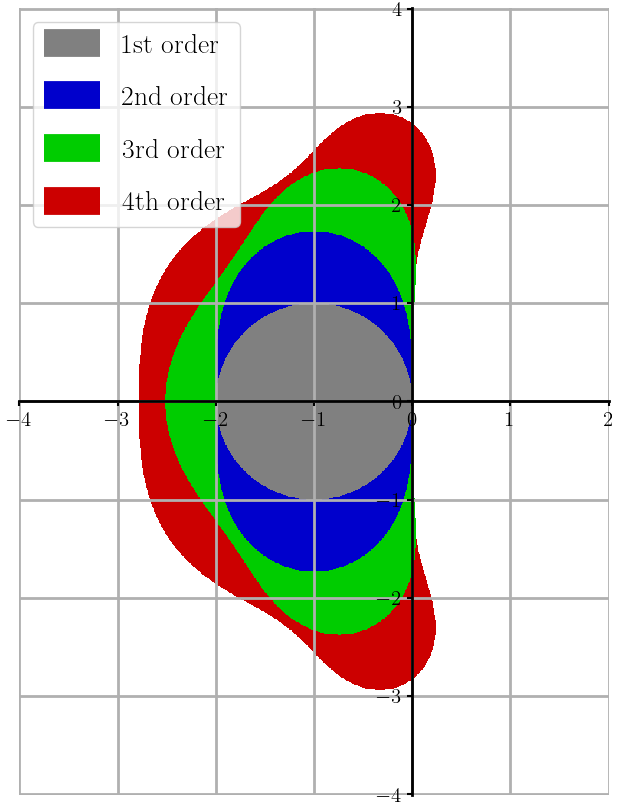
\includegraphics[width=.45\textwidth]{figures/rk_stab.png}
          \caption{Stability regions (in color) of the four first order Runge--Kutta methods.}
          \label{fig:rk_stab}
        \end{figure}

        \paragraph{}
        We can see that Runge--Kutta methods are not A-stable, and they do not have a large stability region.
        Increasing the order of the method does increase the stability region, but not enough for our applications.
        Practically, this impose the use of small time steps, which is agreeable for unsteady computations but not for our steady ones.
        If ont iteration of the method is inexpensive, the total number of iterations needed to reach the steady solution will make the overall computation too costly.


      \subsection{Adams--Bashforth methods}

        \paragraph{}
        We could try to use other explicit methods, such as the multi step Adams--Bashforth methods.
        The $k$th order Adams--Bashforth method uses the last $k$ computed steps to find the next one.
        One can indeed check that the index $k$ designating the method also corresponds to its order \cite{HairerNorsettWanner1993}.

        \paragraph{}
        The idea is to apply a Lagrange interpolation of the function $\operatorname{G}$ from equation (\ref{eq:init_value_ode}) in the $k$ last computed points, and then replace $\operatorname{G}$ with the interpolation polynomial when integrating from $t_n$ to $t_{n+1}$.
        Contrary to the Runge--Kutta methods, as we reuse previous information, a single $\operatorname{G}$ evaluation is required at each step.
        The cost of one iteration of the Adams--Bashforth method is then really cheap \PS{(reformuler)}.
        The stability analysis for such methods is a bit more complex \cite{HairerNorsettWanner1993, HairerWanner1996}, and so we show the result that we obtained numerically on figure \ref{fig:ab_stab} without \PS{faire le calcul : deriving the calculus ?}.
        The conclusion is even worse than with the Runge--Kutta methods, as the stability region decreases as the order increases.
        The Adams--Bashforth can reach a high order of accuracy while staying computationally inexpensive, but they lack drastically of stability, and that is why they are often not used in computational fluid dynamics computations.
        More generally, an explicit multi step method cannot be A-stable \cite{Dahlquist1963}.

        \begin{figure}
          \centering
          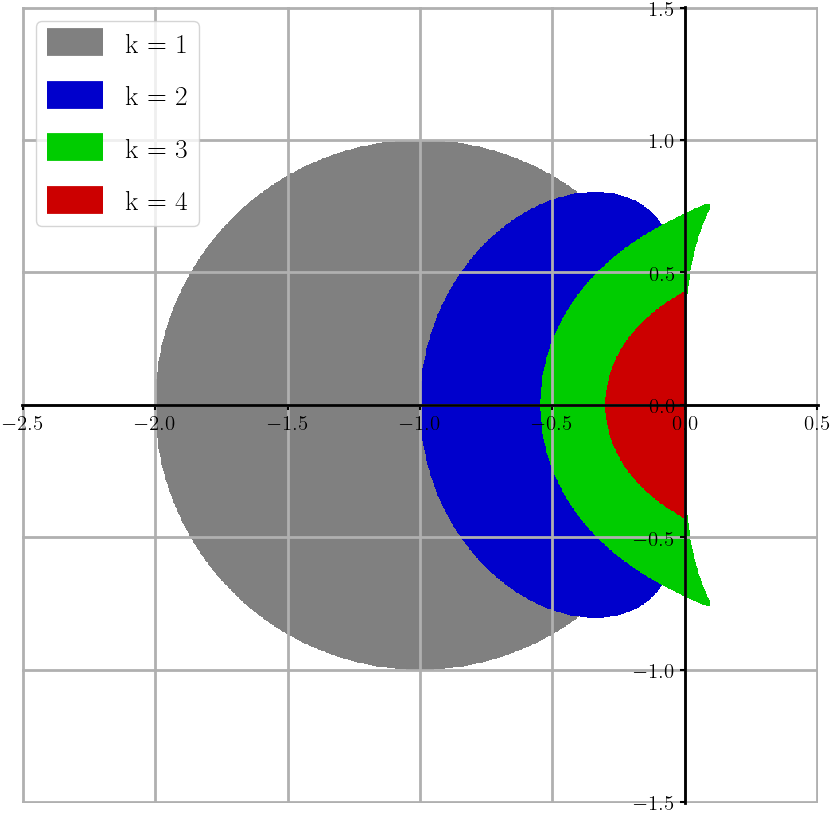
\includegraphics[width=.6\textwidth]{figures/ab_stab.png}
          \caption{Stability regions (in color) of the four first Adams-Bashforth methods.}
          \label{fig:ab_stab}
        \end{figure}


    \subsection{Implicit methods}

      \paragraph{}
      We explained in the previous section why explicit time integration methods are not suited for our applications.
      It is then natural to look at implicit methods.
      Contrary to the explicit methods, implicit methods do not give the looked for solution right away, but as the solution of a specific equation.
      The name is appropriate: the next state is not given explicitly but implicitly.


      \subsubsection{Implicit Euler method}

        \paragraph{}
        The implicit Euler method is the equivalent of the explicit Euler method but on the implicit side.
        It is quite similar, as it consists in integrating equation (\ref{eq:init_value_ode}) assuming the function $\operatorname{G}$ is constant, but this time equal to $\operatorname{G}\left(\Xi_{n+1}\right)$.
        We then have:
        \begin{equation}
          \Xi_{n+1} = \Xi_n - \Delta t \operatorname{G}\left(\Xi_{n+1}\right)
          \Leftrightarrow \Xi_{n+1} - \Xi_n + \Delta t \operatorname{G}\left(\Xi_{n+1}\right) = 0
        \end{equation}
        and the next state $\Xi_{n+1}$ is given as the solution of a nonlinear problem, the root of a nonlinear function.

        \paragraph{}
        After checking that this is a first order method, we can also do the stability analysis to find the corresponding function $g\left(z\right) = \left(1 - z\right)^{-1}$, that gives a stability region equal to the whole complex plane minus the closed unity disk centered in 1.
        Therefore this method is A-stable.


      \subsubsection{Implicit Runge--Kutta methods}

        \paragraph{}
        Runge--Kutta methods can also be implicit methods.
        This happens when the quadratures use points that have not already been computed.
        In other words, this corresponds to a full $A$ matrix in the butcher tableau, where it is strictly lower triangular for explicit Runge--Kutta methods.
        This also means that any step of the Runge--Kutta method may be used in any other step, and therefore we may have to simultaneously solve an implicit system of equations.
        This may lead to awfully expensive methods, and therefore users tend to restrict themselves to some particular methods.

        \paragraph{}
        Despite their cost, implicit Runge--Kutta methods can be appealing.
        The main reason is that they can easily achieve a high order of accuracy.
        For example, the methods based on Gauss--Legendre quadratures achieve an order $2k$ with $k$ steps, and they are all A-stable \cite{Iserles2008}.
        Theoretically this means we can achieve an arbitrary high order while keeping the stability quality with these methods.
        However, users usually stop at the 3-stage 6th order method, as the computational cost tend to be too much for higher order methods.

        \paragraph{}
        When applying the stability analysis to a Runge--Kutta method, we can derive the function $g$ using the arrays $A$, $b$ and $c$:
        \begin{equation}
          g\left(z\right) = 1 + z \transpose{b} \left(\operatorname{Id} - zA\right)^{-1} \transpose{\left(1, \dots, 1\right)} \ .
        \end{equation}
        We will not try to show the corresponding stability regions as there are too many methods possible.
        Instead, we will review some of the most frequent from the literature.

        \paragraph{Diagonally Implicit Runge--Kutta methods}
        The Diagonally Implicit Runge--Kutta methods \cite{Alexander1977}, or DIRK methods, are Runge--Kutta methods with a lower triangular matrix $A$.
        Then, each step is given as an implicit problems using the already known steps.
        The difference is that instead of solving a full implicit system, we just need to solve each implicit step successively.
        This help drastically reduce the cost of the method.
        Furthermore, if all quadrature coefficient $a_{ii}$ are equals, as we invert at each step the matrix $\operatorname{Id} + a_{ii} \Delta t \frac{\mathrm{d} \operatorname{G}}{\mathrm{d} \Xi}\left(\Xi_n\right)$, this can help the linear solve.
        This variant is called Singly Diagonally Implicit Runge--Kutta methods (SDIRK) \cite{HairerWanner1996}.

        \paragraph{Rosenbrock methods}
        Rosenbrock methods are also called linearly implicit Runge--Kutta methods.
        \PS{TODO ?}


      \subsubsection{Backward differentiation formula}

        \paragraph{}
        As we extended the explicit Runge--Kutta methods to implicit methods, we can also extend the Adams-Bashforth method to an implicit one.
        When interpolating the function $\operatorname{G}$, we add ont point to the Lagrange interpolation: the point we want to compute.
        This new method is called an Adams-Moulton method.
        However, the stability region of Adams-Moulton is quite narrow, as they were originally not made for stiff equations \cite{Iserles2008}.
        This is why the BDF methods were introduced.
        Contrary to Adams-Bashforth and Adams-Moulton methods, they use the Lagrange interpolation of the solution $\Xi$ instead of the function $\operatorname{G}$.
        Then, we can replace the time derivative of the solution by the time derivative of the interpolating polynomial, and evaluate this new equality at the next time step $t_{n+1}$.
        This gives an implicit equation we need to solve to get $\Xi_{n+1}$.
        The name of those methods come from the fact that if we use a constant time step between iterations, this equation can be written using the differentiating operator defined by $\nabla^0 \square_i = \square_i$ and $\nabla^{j+1} \square_i = \nabla^j \square_i - \nabla^j \square_{i-1}$:
        \begin{equation}
          \sum_{i=1}^k \frac{1}{i} \nabla^i \Xi_{n+1} + \Delta t \operatorname{G}\left(\Xi_{n+1}\right) = 0
        \end{equation}

        \paragraph{}
        We can show that the order of the method is equal to the index of the method, corresponding to the number of previous states needed to compute the next one.
        These methods allow for an arbitrary high order without increasing the coast, as the implicit equation is not harder to solve as the order increases.
        However, the stability analysis limits the higher order achievable.
        The stability analysis of the BDF methods can be done numerically.
        At this stage, we can note that the first order BDF method is in fact the implicit Euler method.
        Also, methods of order 7 or higher are unstable, so we can limit our analysis on methods with orders from 1 to 6.
        The corresponding stability regions are satisfying, as can be seen on figure \ref{fig:bdf_stab}.
        Particularly, the first and second methods are A-stable.
        More generally, there are no A-stable multi steps methods with an order higher than 2 \cite{Dahlquist1963, HairerWanner1996}.

        \begin{figure}
          \centering
          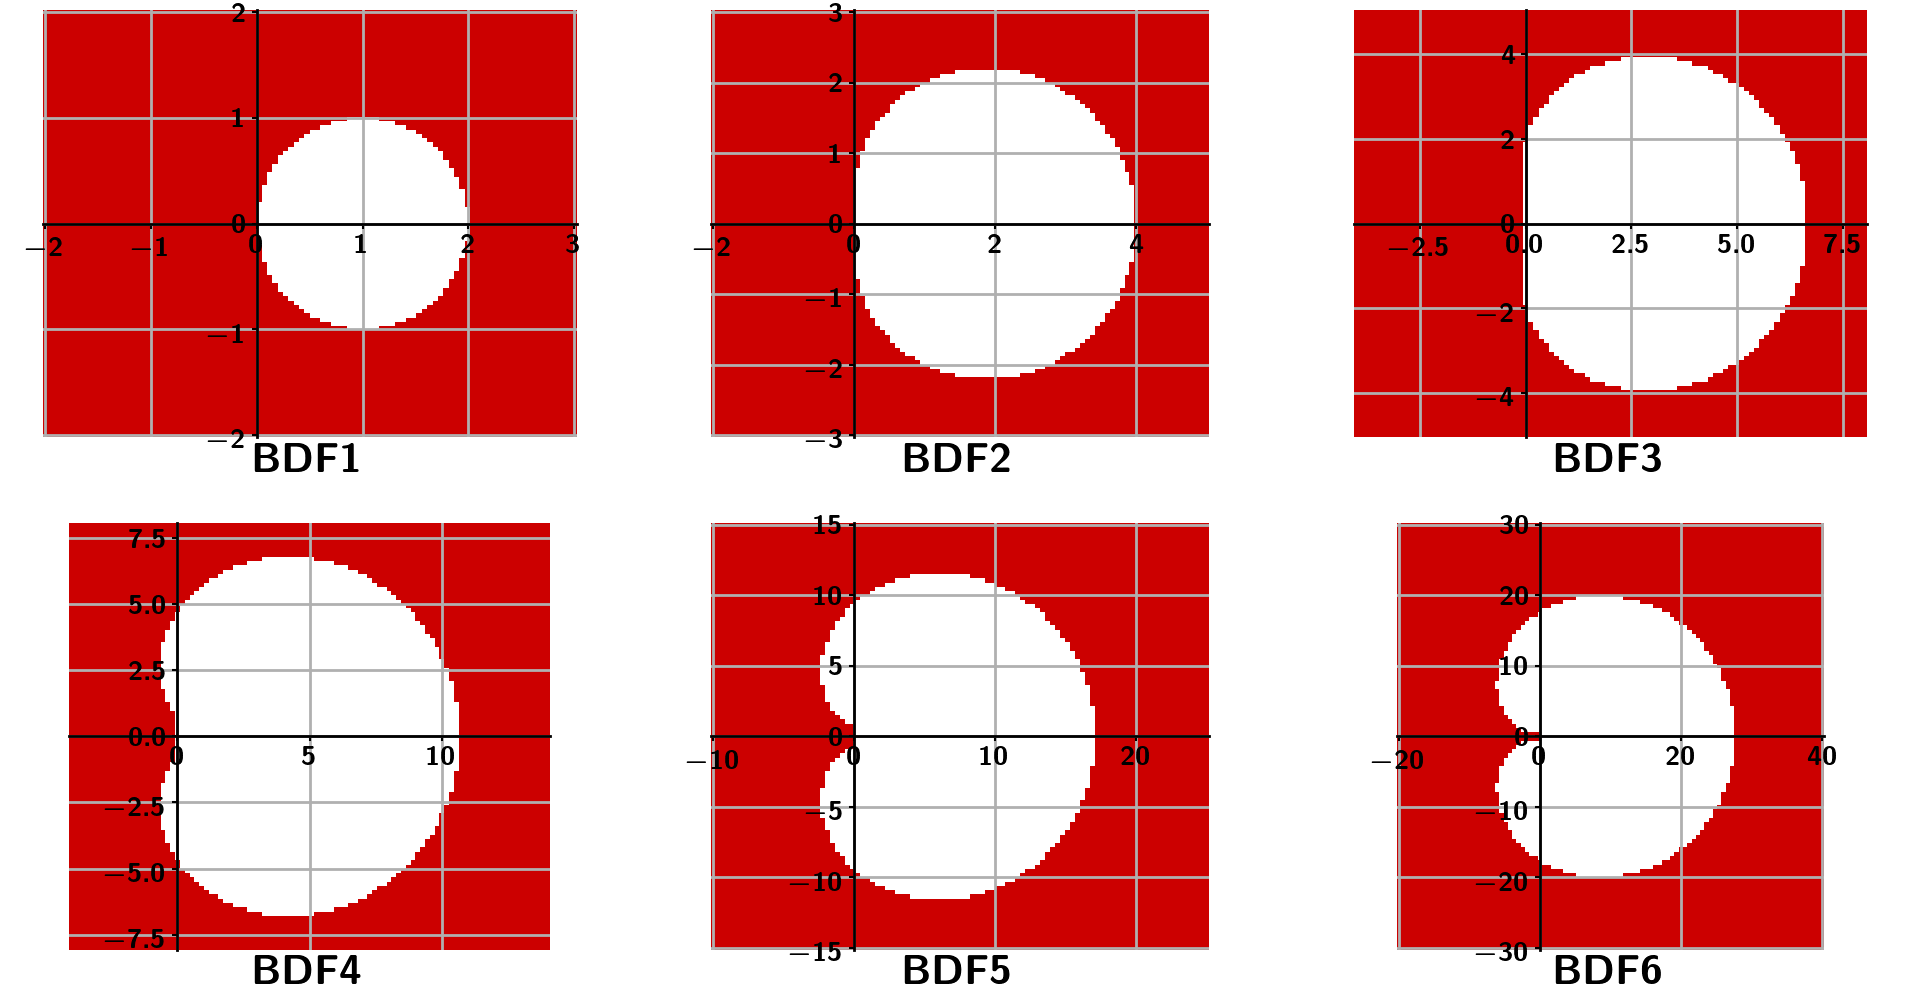
\includegraphics[width=\textwidth]{figures/bdf_stab.png}
          \caption{Stability regions (in color) of the BDF methods.}
          \label{fig:bdf_stab}
        \end{figure}

      \paragraph{}
      This introduction to the classic time integration methods helps us to decide what to do for our solver.
      As we said earlier, we want to solve an ordinary differential equation in order to recover the steady solution, reached after a long time.
      Then, explicit methods that constrain the time step are not well fitted.
      Even if they cost more, in an algorithmic way, implicit methods are indeed the best choice for our stiff equations.
      It is often better to do a single expensive iteration over a large time step with an implicit method, than making a lot of inexpensive iterations over small time steps with an explicit method.
      This is finally why we will continue working with the A-stable implicit Euler method.
      This method is at the base of all other implicit methods, as they can be seen as small variations of the implicit Euler methods.
      Choosing it is also smart as updating it into an other implicit time integration method will not require too much work.
      \PS{et parce que c'est dans CHARME ?}


  \section{Implicit methods framework}
  \PS{Revoir structure}


    \subsection{Methodology of the implicit time integration}

      \paragraph{}
      As we explained in the previous section, implicit time integration methods give the next state as the solution of a nonlinear equation, or a system of nonlinear equations.
      If we want to use implicit methods, we then need to be able to solve a nonlinear problem.
      We will continue our discussion using the implicit Euler method, but everything can easily be adapted for any other implicit method.
      For Diagonally Implicit Runge--Kutta methods, we apply the nonlinear solve successively for each step.
      For BDF methods, we apply the nonlinear solve on a slightly different equation.


      \subsubsection{From a nonlinear problem \dots}

      	\paragraph{}
      	We can use Newton's method to solve a nonlinear problem of the form:
      	\begin{equation}
      		\tilde{f}\left(\Xi_{n+1}\right) = 0 \ .
      	\end{equation}
        Equivalently, as we work here for a single $n$ at a time, we could express this equation in terms of the increment $x = \Xi_{n+1} - \Xi_n$:
        \begin{equation}\label{eq:nonlinear}
      		f\left(x\right) = 0 \ .
      	\end{equation}
        Newton's methods starts from an initial guess $x_0$.
        We usually take $x_0 = 0$ as it equivalent to take $\Xi_n$ as an initial guess for $\Xi_{n+1}$.
        The method will then iterate to approximate the solution of equation (\ref{eq:nonlinear}).

        \paragraph{}
        At each step of Newton's method, we linearise \PS{au premier ordre} in the current estimation $x_i$ the nonlinear function $f$ evaluated  in the next iteration $x_{i+1}$ and we set this linearisation equal to 0, the desired value:
        \begin{equation}\label{eq:nonlinear_linearised}
          f\left(x_{i+1}\right) \approx f\left(x_i\right) + f'\left(x_i\right) \left( x_{i+1} - x_i \right) = 0
        \end{equation}
        This gives a linear problem of which $x_{i+1}$ is the solution.
        \PS{Refs sur méthode de Newton ?}


      \subsubsection{\dots to a linear one}

        \paragraph{}
        We can rewrite equation (\ref{eq:nonlinear_linearised}) into the classic linear problem \PS{notation x déjà utilisée}:
        \begin{equation}\label{eq:linear}
          Ax = b
        \end{equation}
        where we can identify $A = f'\left(x_i\right)$, $b = -f\left(x_i\right)$ ans $x = \left( x_{i+1} - x_i \right)$.
        A lot of methods were conceived to solve such linear problems, and we will discuss later how we will handle it.


      \paragraph{}
      To sum up, we started from the partial diferential equation (\ref{eq:pde}) arising from the physical model.
      With a spatial discretisation method, and after choosing an initial value, this transforms into an ordinary differential equation (\ref{eq:init_value_ode}).
      For stability reasons, we decided to use implicit time integration methods.
      Iteratively, such methods are going to produce one or several nonlinear problems of the form of equation (\ref{eq:nonlinear}).
      The newton's method used to solve such problems is going to produce a succession of linear problems of the form of equation (\ref{eq:linear}).
      This complicated sequence of operation describes the time integration procedure used in our solver to find the solution of steady problems.
      It is schematised on figure \ref{fig:steady_solve}, where the blue circles correspond to the problems being solved, while green circles correspond to the methods used to solve them.
      In this theses, we are interested in the non grayed out parts.

      \begin{figure}
        \centering
        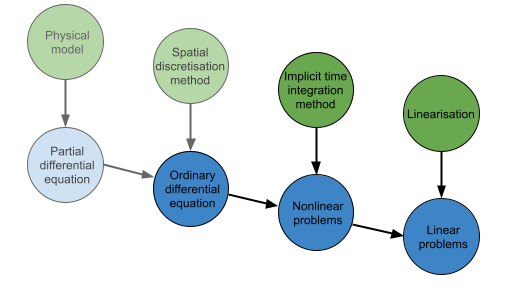
\includegraphics[width=.8\textwidth]{figures/steady_solve.png}
        \caption{Procedure used to find the solution of steady problems.}
        \label{fig:steady_solve}
      \end{figure}


    \subsection{Nonlinear solver}


    \subsection{Linear solver}

      \paragraph{}
      We want to be able so solve efficiently linear systems like (\ref{eq:linear}).
      We additionally assume that $A$ is an invertible matrix.
      Let us note the size of the linear system $N$.
      This size is quite large in our typical applications, but the linear system is sparse.
      This means that the coefficients of the matrix $A$ are mostly zeros.
      This is because a coefficient in the matrix $A$ corresponds to a link between two degrees of freedom.
      For the spatial discretisation methods we use, a cell depends on a small number of neighboring cells, and therefore a degree of freedom does is not linked with most of the others \PS{(c'est clair ?)}.
      Such sparse matrices can be seen on figure \ref{fig:sparse}.
      Using the sparsity of the matrix is essential, as it would not be possible to store it as a dense matrix in the memory of a computer.
      Instead, we use some clever formats such as the Compressed Sparse Row format \cite{Saad2003}.
      Some operations such as matrix vector products are more efficiently done using such formats.

  		\begin{figure}
  			\centering
  			\begin{subfigure}[t]{0.3\textwidth}
  				\centering
  				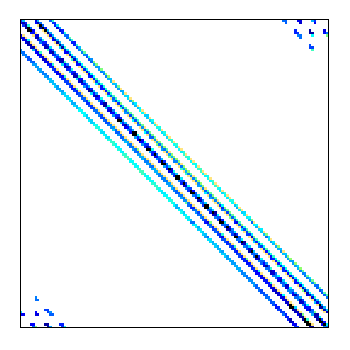
\includegraphics[width=\textwidth]{figures/GT01R.png}
          \caption{GT01R: 2D inviscid flow in the inter-blade channel of a linear cascade turbine.}
  				\label{fig:sparse.GT01R}
  			\end{subfigure}
  			\hfill
  			\begin{subfigure}[t]{0.3\textwidth}
  				\centering
  				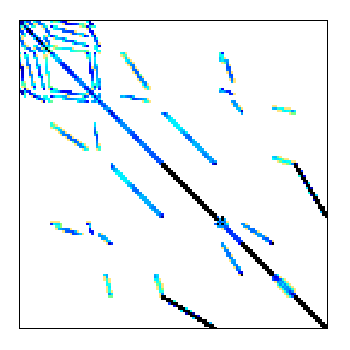
\includegraphics[width=\textwidth]{figures/HV15R.png}
  				\caption{HV15R: 3D RANS simulation of an engine fan.}
  				\label{fig:sparse.HV15R}
  			\end{subfigure}
  			\hfill
  			\begin{subfigure}[t]{0.3\textwidth}
  				\centering
  				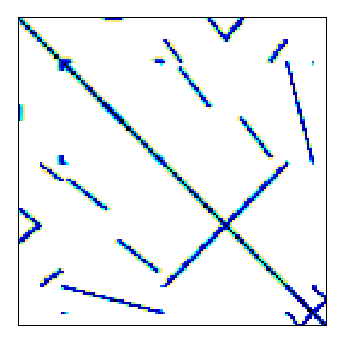
\includegraphics[width=\textwidth]{figures/RM07R.png}
  				\caption{RM07R: 3D viscous flow in a jet engine compressor.}
  				\label{fig:sparse.RM07R}
  			\end{subfigure}
  			\caption{Matrices from various CFD simulations \cite{PacullAubertBuisson2011} using a Finite Volumes method. Colored points correspond to nonzero values.}
  			\label{fig:sparse}
  		\end{figure}

      \paragraph{}
      Many methods exists to solve linear problems.
      Some are even taught in school, such as the Gaussian elimination.
      Such methods are called direct methods, as they first do some work and then find directly the exact solution of the problem.
      But for problems with huge size as the ones we encounter in computational fluid dynamics, the amount of work is too much to be computed with today's means.
      It would take too much time as well as too much memory.
      Instead, we can use iterative methods.
      An iterative method starts from an initial guess $x_0$ and produces as it iterates a supposedly better estimation of the solution $x_n$.
      The subscript $n$ has nothing to do with the subscript used to identify the iterates of the time integration method: we work at a given fixed time step here.
      We can then decide when to stop the method, whether the solution estimate is good enough or the solve is taking too much time.
      Iterative methods are the most well fitted to solve large sparse linear problems, and they are the preferred solution in computational fluid dynamics.

      \paragraph{}
      Among the iterative methods are what could be called the "classic" methods, or relaxation.
      They are the Jacobi, Gauss--Seidel or Successive Over Relaxation methods.
      They decompose the matrix into $A = M - N$ with $M$ a matrix easily invertible.
      The choice of $M$ depends on the method.
      Then, starting from a given $x_0$, at each step we compute $x_{n+1} = M^{-1} \left( N x_n + b \right)$.
      Those methods are often deemed not efficient enough for computational fluid dynamics applications.
      They are often used, however, as preconditioning methods, as we will see later.

      \paragraph{}
      Another class of iterative methods is becoming the standard for computational fluid dynamics: the Krylov subspace methods.
      A Krylov subspace method projects the linear problem (\ref{eq:linear}) on a smaller linear subspace called Krylov subspace.
      The obtained smaller system is then solved, much more easily.
      The cleverness resides in the fact that those Krylov subspaces are \PS{emboités}, and each iteration reuses the information obtained in the previous ones.

      \paragraph{}
      In the following, we note at iteration $n$ the residual $r_n = b - A x_n$.
      Practically, we keep $n \ll N$ so that the cost of the method stays reasonable, but this does not change the following.
      The corresponding Krylov subspaces are defined as:
  		\begin{equation}
  			\krylov[A, r_0]{n} = \operatorname{Vect}\left( r_0, A r_0, \dots, A^{n-1} r_0 \right) \ .
  		\end{equation}
      Then, we seek the next iterate in $\krylov{n}$ satisfying a Petrov--Galerkin condition \cite{SimonciniSzyld2007}:
  		\begin{equation}
  			x_n \in x_0 + \krylov[A, r_0]{n} \quad \textrm{such as} \quad r_n \perp \mathcal{L}_n
  		\end{equation}
      where $\mathcal{L}_n$ is a linear subspace with dimension $n$.
      For example, $\mathcal{L}_n = \krylov{n}$ corresponds to a Galerkin condition, and $\mathcal{L}_n = A \krylov{n}$ is a minimum residual condition.

      \paragraph{}
      To construct the growing Krylov subspace, we can use the Arnoldi iteration \cite{TrefethenBau1997}.
    \paragraph{}
    There are many Krylov subspace methods that can solve a linear problem, characterised by the choice of $\mathcal{L}_n$.
    The minimal residual condition gives the GMRES method \cite{SaadSchultz1986}, vastly used in computational fluid dynamics \cite{FrancoCamierAndrejEtAl2020} and other fields of numerical simulations \cite{ErnstGander2012, Mercier2015}.
    Its main advantage is that even if its iterations may be slightly more expensive than other methods such as the Bi-CGSTAB method \cite{Vorst1992, TrefethenBau1997}, the residual norm is minimised and the error is then decreasing as the method iterates \PS{phrase pas claire ?}.
    The GMRES method already exists in our solver and is often used.
    Because it is discussed a lot in the literature, many variants and enhancements were developed \cite{Vasseur2016}.
    For those reasons, we decided to keep the GMRES method as the base of our linear solver.
    \subsection{Evaluating the Jacobian matrices}

      \paragraph{}
      At this point, we know how to evaluate the function $f$ from equation (\ref{eq:nonlinear}), that is often expressed as a linear combination of previous states and $\operatorname{G}$ evaluations, where $\operatorname{G}$ is the function introduced in equation (\ref{eq:init_value_ode}), the function from our starting ordinary differential equation.
      On the other hand, computing its derivative with regard to $x$ is a different story.
      This derivative $f'\left(x\right)$ uses the Jacobian matrix of the function $\operatorname{G}$.
      As the function $\operatorname{G}$ comes from the spatial discretisation method applied to the original partial differential equations (\ref{eq:pde}), is is complex, not in the sense of imaginary numbers but of complicated.
      The underlying algorithm is hard to fully understand and to write, and the numerical evaluation us usually expensive.
      Finding an algorithm that computes the exact Jacobian matrix analytically would amount to too much work in out industrial software.
      We must use other alternatives to get the Jacobian matrix we need for our Newton's method.

      \paragraph{}
      An idea would be to use \emph{Automatic Differentiation} \cite{Griewank2000}.
      This means to give the source code of the $\operatorname{G}$ function to some software \cite{HascoeetPascual2012}, that gives in return a way to compute its Jacobian matrix.
      One advantage of this method is that the cost of derivating the function is done only once, at software compilation.
      After that, computing the Jacobian matrix amount to calling a function.
      Another advantage is that the given Jacobian is supposedly exact, contrary to some alternatives we will discuss later.
      For those reasons, Automatic Differentiation is today being used in actual computational fluid dynamics softwares \cite{BilanceriBeuxElmahiEtAl2011, KenwayMaderHeEtAl2019}.
      In our software, using Automatic Differentiation did seem too hard and therefore we looked at other methods instead.
      \PS{Plus justifier ? Reformuler ?}

      \paragraph{}
      A possible idea is to use an approximation of the Jacobian matrix that is inexpensive to compute.
      We said that the function $\operatorname{G}$ comes from the second order or higher Finite Volume method used as the spatial discretisation method.
      We can take the function $\operatorname{G}_1$ given by the first order corresponding method, and use its Jacobian matrix instead.
      Indeed, computing $\operatorname{G}_1$ is inexpensive in comparaison to $\operatorname{G}$, and the same goes for the corresponding Jacobian matrices.
      Going further, we could also approximate the Jacobian matrix of $\operatorname{G}_1$: when $\operatorname{G}$ uses some complex models such as turbulence models, it is often decided to not include those models contributions to the Jacobian matrix, for complexity and stability reasons \PS{ref ici}.
      This is what is done originally in out in-house solver: using a cheap low order approximation of the Jacobian matrix.

      \paragraph{}
      An other idea is to group the Newto



    \PS{Nécessité de calculer des Jacobiennes --> JFNK}

    \PS{Résolution système linéaire --> GMRES}

    \PS{Préconditionnement sans utiliser la matrice --> FGMRES}
